\documentclass[conference]{IEEEtran}
% \IEEEoverridecommandlockouts
% The preceding line is only needed to identify funding in the first footnote. If that is unneeded, please comment it out.
\usepackage{cite}
\usepackage{amsmath,amssymb,amsfonts}
\usepackage{algorithmicx}
\usepackage{url}
\usepackage{setspace}
\usepackage{algorithm}
\usepackage{multicol}
% \usepackage{arevmath}
\usepackage{algpseudocode}
\algrenewcommand\Return{\State \algorithmicreturn{} }%
\algnewcommand{\LineComment}[1]{\State \(//\) #1}

\usepackage{dblfloatfix}
\usepackage{graphicx}
\usepackage{textcomp}
\usepackage{xcolor}
\def\BibTeX{{\rm B\kern-.05em{\sc i\kern-.025em b}\kern-.08em
    T\kern-.1667em\lower.7ex\hbox{E}\kern-.125emX}}
\begin{document}

\title{Dynamic Reconfiguration and Resource Provisioning in Pi Clusters % *\\
% {\footnotesize \textsuperscript{*}Note: Sub-titles are not captured in Xplore and
% should not be used}
% \thanks{Identify applicable funding agency here. If none, delete this.}
}

\author{\IEEEauthorblockN{Rohit Das}
\IEEEauthorblockA{\textit{Dept. of Electrical Engineering and Computer Science} \\
\textit{Indian Institute of Technology Bhilai}\\
Raipur, India \\
rohitd@iitbhilai.ac.in}
\and
\IEEEauthorblockN{Dr. Subhajit Sidhanta}
\IEEEauthorblockA{\textit{Dept. of Electrical Engineering and Computer Science} \\
\textit{Indian Institute of Technology Bhilai}\\
Raipur, India \\
subhajit@iitbhilai.ac.in}
% \and
% \IEEEauthorblockN{3\textsuperscript{rd} Given Name Surname}
% \IEEEauthorblockA{\textit{dept. name of organization (of Aff.)} \\
% \textit{name of organization (of Aff.)}\\
% City, Country \\
% email address or ORCID}
% \and
% \IEEEauthorblockN{4\textsuperscript{th} Given Name Surname}
% \IEEEauthorblockA{\textit{dept. name of organization (of Aff.)} \\
% \textit{name of organization (of Aff.)}\\
% City, Country \\
% email address or ORCID}
% \and
% \IEEEauthorblockN{5\textsuperscript{th} Given Name Surname}
% \IEEEauthorblockA{\textit{dept. name of organization (of Aff.)} \\
% \textit{name of organization (of Aff.)}\\
% City, Country \\
% email address or ORCID}
% \and
% \IEEEauthorblockN{6\textsuperscript{th} Given Name Surname}
% \IEEEauthorblockA{\textit{dept. name of organization (of Aff.)} \\
% \textit{name of organization (of Aff.)}\\
% City, Country \\
% email address or ORCID}
}

\maketitle
\thispagestyle{plain}
\pagestyle{plain}

\begin{abstract}
In a resource-constrained computing setup, efficient allocation of resources is essential. Edge clusters consisting of small, single-board computers are cheaper, easily deployable and re-configurable. During unavailability of cloud services or intermittent network coverage, edge clusters can be helpful. To enable feasible usage of such clusters, algorithms to manage failure and overloading are essential. Most of the related works lack  in the regard of using ARM devices for such clusters.
\end{abstract}

\begin{IEEEkeywords}
edge computing, raspberry pi, distributed systems, resource-constrained, resource provisioning
\end{IEEEkeywords}

\section{Introduction}

With the emergence of cloud computing, computational resources have become more flexible and easily available. Be it deep learning analytical models, online software subscriptions or data storage, cloud computing is the most popular choice. However, using cloud services require stable bandwidth, SLA's promising competitive low values of downtime and fast results. Where cloud fails, edge computing comes in. Using single-board computers to create an edge cluster, we can offload cloud services to the edge, speeding up data processing and lowering transmission latency. Such lightweight clusters need to have algorithms in place to manage node failures, overloading and reconfiguration and be in tandem with quality of cloud services.

Single-board computers like Raspberry Pi usually come with a quad-core processor and at most 4GB of RAM. Nowadays, in the advent of data analytics, the above-mentioned resources are too less for a single node to handle vast amounts of data. So, we are faced with the following problems:
\begin{itemize}
    \item To enable fast processing of a huge in-stream of data, either the rate of data fed into the cluster must be regulated, or the data stream must be parallelized amongst multiple nodes.
    \item Some nodes will be overburdened with processes taking up a lot of resources, like applications involving deep-learning or neural networks, object-recognition from a live video feed, so efficient load-balancing algorithms are essential.
    \item In case of failure of a node, container running on the failed node must be migrated before-hand to a standby node, and the new node must be up and running with as less downtime as possible.
\end{itemize}

\section{Related Works}

Live migration intends to transfer user control or a process from one node to another in a cluster in case of failures or crashes. While live migration is good and suitable for systems set up over LAN having bandwidths in the range of 1-40 Gbps, VM hand-off \cite{elephant} focuses mainly on the edge, having a WAN connection of bandwidth 5 to 25 Mbps.

The process of VM hand-off \cite{elephant} can be broken down into 3 parts: \textbf{delta encoding}, \textbf{deduplication} and \textbf{compression}. Each step of the optimizing process is a module in the VM Hand-off pipeline. The aim is to send only the difference between the modified data in the source VM and the base VM at the destination. The pipeline switches between algorithms to make the best use of both the CPU cores and the network bandwidth.

Redundancy live migration \cite{redun_mig} has been shown to be a significant improvement over the pre-copy, post-copy or the hybrid live migration algorithm. 
% It works as follows:
% \begin{itemize}
%     \item When migration is to start, packets from client are rerouted to the destination server, which buffers them and also sends them over to the source server.
    
%     \item Source server creates a checkpoint when migration starts, i.e. it creates a copy of the container at the current state, and them starts logging further changes in CPU state, memory state, etc. after the checkpoint is triggered.
    
%     \item Source server then sends over the copy of the container at checkpoint to the destination server, followed by the logs, when downtime occurs. The destination server replays the logs and syncs with the source server.
    
%     \item The destination server then plays back all the buffered packets from the client and starts serving the client, thus migration being complete.

% \end{itemize}

% \begin{figure}[htbp]
% \centerline{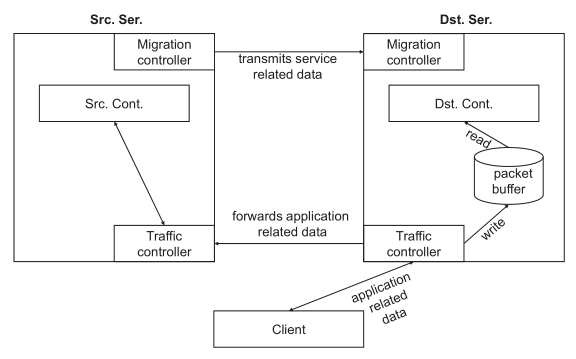
\includegraphics[width = 0.4 \textwidth]{./img/redun_mig.png}}
% \caption{\label{fig:redun_mig} Redundancy Migration High-Level Architecture. \cite{redun_mig}}
% \end{figure}

% The big takeaway here is that the algorithm is network, application or platform agnostic, but it still needs a fixed and minimum bandwidth to send over the container copy, and keep downtime to a specified minimum, as agreed in the SLA (Service-Level Agreement). Also, with ARM devices having low resources, implementing this algorithm will not feasible.

Service migration reduces service latency, and user applications are migrated to the closest MEC(Mobile Edge Clouds) only when it has benefits surpassing the negative effects of downtime. The migration is performed by sending files synchronously over the network. Meaning, only files which have changed significantly in comparison to the destination MEC are sent over. To optimize the amount of data sent out during migration, a three-layered approach \cite{migration_mec} is used. \textbf{Instance layer} migration consists of migrating only application-specific information like the running state of the application. \textbf{Application layer} is involved when the entire application is not found at the destination MEC, and the same is cloned from the source. The topmost \textbf{Base layer} is only involved when the container or VM used itself is not present in the destination, and needs to be packaged and sent from the source.

% \begin{itemize}
%     \item Instance layer: This consists of migrating only the application-specific information, like the running state of the application, metadata specific to the user, etc.
    
%     \item Application layer: If the application is not found in the destination MEC, the application is cloned from the source, all states and memory data are stores in one or multiple files, and migrated.
    
%     \item Base layer: The guest OS and kernel, etc. are packaged and sent over in this layer. Normally this level of migration is not required since all MECs contain a copy of the guest OS and kernel.
% \end{itemize}

% \begin{figure}[htbp]
% \centerline{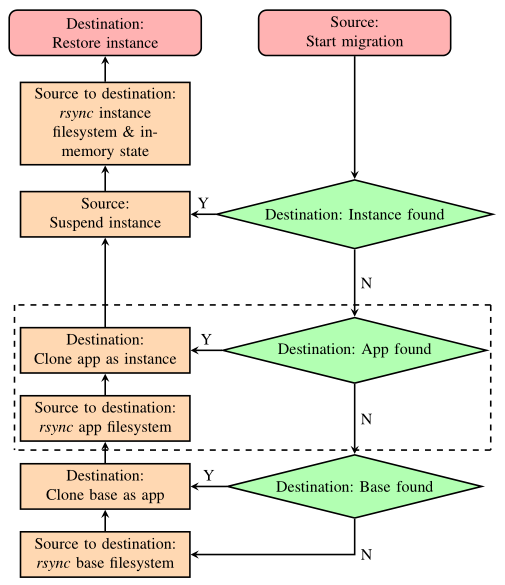
\includegraphics[width = 0.4 \textwidth]{./img/migration1.png}}
% \caption{\label{fig:migr_mec} Flow chart of the migration mechanism for live- migrating with the three-layer model, where \textit{rsync} is used for incremental file synchronization. \cite{migration_mec}}
% \end{figure}

Dynamic Provisioning of resources \cite{dynamic} for a resource-constrained cluster will be helpful to deal with situations like flash crowds, when a sudden amount of huge traffic overwhelms the cluster and fast enough to rearrange the topography of the cluster nodes to accommodate for the sudden surge. The cluster nodes can be tiered to enable handling of the computations and requests at multiple stages. Predictive and Reactive provisioning \cite{daniel2011prediction} can handle flash crowds or deviations from predicted long-term behaviour. Analytical models to allocate servers to a tier based on the estimated workload and accounting for multiple requests that comprise a session and the stateful nature of session-based Internet applications will also help in handling surges.
% through the following ways:
% \begin{itemize}
%     \item Predictive and Reactive provisioning \cite{daniel2011prediction} to handle flash crowds or deviations from predicted long-term behaviour.
%     \item Analytical model to allocate servers to a tier based on the estimated workload.
%     \item Accounting for multiple requests that comprise a session and the stateful nature of session-based Internet applications.
% \end{itemize}

% \begin{figure}[htbp]
% \centerline{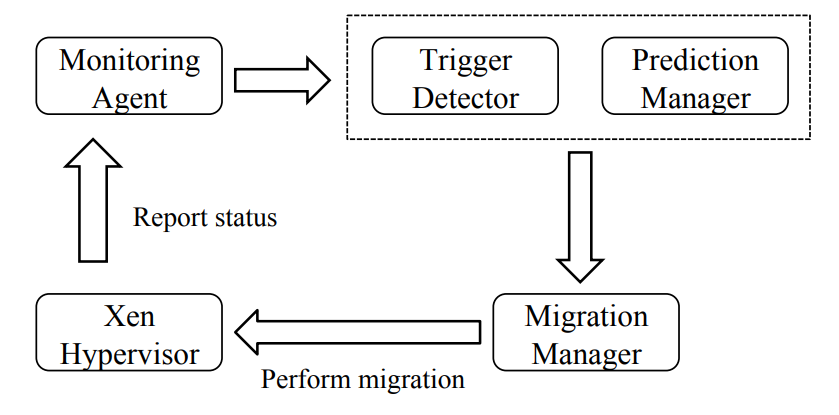
\includegraphics[width=0.4 \textwidth]{./img/load_bal.png}}
% \caption{\label{fig:load_bal} Architecture of Reactive-Predictive Load-Balancer \cite{daniel2011prediction}}
% \end{figure}

% Most of the works cited above involved implementations and system setup consisting of commomplace computer systems having adequate resources, except for MECs. Even then, edge clusters consisting of single-board chip computers have not been used to perform delta VM handoff, with containers running on each node.

% Monitoring the cluster for fault-tolerance and overloading will be essential. YourKit Java Profiler \cite{yourkit2010yourkit} can be used as it is lightweight and will be adequate for the resource-constrained cluster.

\section{Cluster Provisioning and Reconfiguration}

Using single-board chips with low resources make the cluster prone to overloading and failures. Reconfiguring the network in case of node failures, and optimal provisioning of nodes for more intensive computations, as well as scaling down when not needed, is essential for the edge cluster.

Linux Containers (LXC) will be running on each node in the cluster. VMs will not be suitable for single-chip boards that we will be using as VMs take up more resources than containers, and hence more bandwidth will be needed to exchange data among nodes.

There will be two parts to the algorithm: failure handling and overload management. The entire cluster will be segregated into two parts - master cluster, and worker cluster. The master cluster will consist of nodes which can be assigned as pseudo-masters, or super peers. The master node will be handling the worker cluster, consisting of worker nodes. Experiments have shown that having a master node with at least 4 GB RAM prevent the node from crashing due to overload.

\subsection{Node Failure Handling}

Any node may fail due to random crashes, overloading or environmental factors. Each worker node will have an associated standby node to fall back on in case of node failure. Frequent delta migration of data encapsulated by containers among nodes will prevent data loss and mitigate downtime.

The master cluster, containing the master nodes, as well as the worker cluster, containing the worker nodes, will be having a replication factor of $n + k$, $n$ being the cluster size of each type. Each worker node will be allocated a standy node from its respective cluster. Container information like current memory and disk state shall be sent over after every interval of $T$ seconds.

\begin{algorithm}
    \setstretch{1.15}
    \caption{Node Activation on Worker Node}
    \begin{algorithmic}[1]
        \Function{activate{\_}node}{standby{\_}node{\_}MAC}
            \LineComment Checks if active node is down
            \If {time.now() $>$ last{\_}seen + $T$ + $t$}
                \State {send msg(MAC,active{\_}node) to curr{\_}master}
                \LineComment Standby node takes over
                \State {restart container from last{\_}state{\_}recvd}
                \State {send container data to standby node}
                \While {true}
                    \State {send delta{\_}diff(curr{\_}lxc{\_}state, last{\_}state)}
                    \State {last{\_}state $\leftarrow$ curr{\_}lxc{\_}state}
                    \State {last{\_}seen $\leftarrow$ time.now()}
                    \State {sleep ($T$)}
                \EndWhile
            \EndIf
        \EndFunction
    \end{algorithmic}
\end{algorithm}

For the first time, entire container information will be sent over to the standby node. In consecutive intervals, only the delta difference in states of active and standby nodes will be sent over. That way, information sent over the network and overall bandwidth usage can be minimized.

Whena standby node does not receive any information after $T + t$ seconds, $t$ being the failure tolerance interval, it will inform the active master, take over from the failed active node and mark itself as an active node. The master will allocate a standby node from the pool and the new node will pick up from where the failed node left off.

\begin{algorithm}
    \setstretch{1.15}
    \caption{Node Activation on Master Node}
    \begin{algorithmic}[1]
        \Function{activate{\_}node}{standby{\_}node{\_}MAC}
            \LineComment Marks respective active node as down
            \State {active{\_}node $\leftarrow$ hash{\_}list [standby{\_}node{\_}MAC]}
            \State {hash{\_}list [active{\_}node].state = down}
            \For {node in hash{\_}list}
                \If {hash{\_}list [node] == NULL AND\\ hash{\_}list [node].state != down}
                    \State {standby{\_}node{\_}MAC.activate{\_}node (node)}
                    \State exit
                \EndIf
            \EndFor
        \EndFunction
    \end{algorithmic}
\end{algorithm}

For a master node, two nodes will be on standby, and will receive delta differences from the active master. When the active master node fails, a bully leader election will decide the new master node, which will then broadcast its own MAC to the worker cluster.

A list of available nodes with their hostname and MAC will be maintained at every node. It will also contain important information on the nodes like their status (dead or alive), if they are an active or standby node, their corresponding standby or active node, etc. When a worker node fails, only the active master can change its own record. It can broadcast the new node after every $T'$ interval. When a master node fails, the new master node will broadcast itself and the changes in the record, thus reducing bandwidth usage.

\subsection{Node Provisioning through Reconfiguration}

Monitoring the nodes in the cluster can prevent failure due to overloading. Any under-utilized nodes from the cluster can be removed to optimize resource usage. Using YourKit, memory and disk usage can be monitored on each node.

When resource usage is above a certain threshold, the active node can request the active master to add more nodes to the cluster to distribute the jobs and prevent overloading. If two free nodes are found in the pool, the master assigns one as the active node, and the other as a standby node, and adds them both to the cluster.
% Similarly, if resource utilization falls below a threshold, the active node can be put on standby, or taken out of the cluster, to be requisitioned when needed.

\begin{algorithm}
    \setstretch{1.15}
    \caption{Additional Node Allocation}
    % \begin{multicols}{2}
    \begin{algorithmic}[1]
        \Function{allocate{\_}node}{active{\_}node{\_}MAC,stats}
            \LineComment Checks if stats are above threshold
            \If {stats.memory $>$ $Mem_{thresh.}$ OR stats.disk{\_}usage $>$ $Disk_{thresh.}$}
                \State active{\_}node = NULL
                \State standby{\_}node = NULL
               \For {node in hash{\_}list}
                \If {hash{\_}list [node] == NULL AND\\ hash{\_}list [node].state != down}
                    \If {active{\_}node == NULL}
                        \State active{\_}node = node
                    \ElsIf {standby{\_}node == NULL AND node != active{\_}node}
                        \State standby{\_}node = node
                    \Else
                        \State exit
                    \EndIf
                \EndIf
            \EndFor
            \EndIf
        \EndFunction
    \end{algorithmic}
    % \end{multicols}
\end{algorithm}

If only one free node is found, the node will be assigned as an active node and added to the cluster. An existing standby node may be reassigned to this active node. If no free node is found, one of the standby nodes will be assigned as an active node, and a standby node will reassigned from the cluster.

Similarly, when resource usage falls below the lower threshold, nodes can be unassigned to scale-down the cluster. Important info on the node will be broadcast to all workers before taking it out. (How to scale down?)

\section{Experimental Setup and Implementation}

The experimental setup consists of creating a cluster using Raspberry Pi 3 Model B+ single-board computers. Each Pi consists of a 1.4GHz 64-bit quad-core processor, 1GB LPDDR2 SDRAM and 32GB micro-SD cards. Each node is running Raspbian OS based on Linux. The networking is done using wireless LAN, and each node has its own micro-USB charger. A file with the list of MACs of all nodes in the cluster will be maintained in each node. That way, we can easily find the IPs of each node when the cluster starts up.

\begin{figure*}[!b]
% \centerline{
\centering
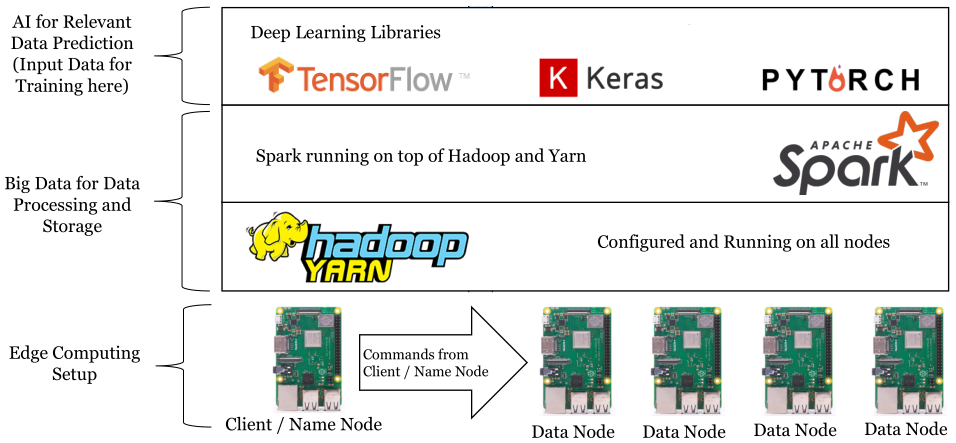
\includegraphics[width = 0.5 \textwidth,]{./img/edge_cluster.png}
% }
\caption{\label{fig:edge_cluster} Edge Cluster Setup using Raspberry Pi}
\end{figure*}


Apache$\textsuperscript{\texttrademark}$ Hadoop$\textsuperscript{\textregistered}$ and Apache Spark$\textsuperscript{\texttrademark}$ are installed in each node to distribute jobs across the cluster. One node is chosen as the name node, which will be responsible for starting HDFS and Yarn across the cluster.

Python libraries like Tensorflow, Keras and Elephas help to distribute Deep Learning tasks across a Spark Cluster. However, since we are starting the cluster from the name node, due to low resources, the jobs start to lag.

% \section{Ease of Use}

% \subsection{Maintaining the Integrity of the Specifications}

% The IEEEtran class file is used to format your paper and style the text. All margins, 
% column widths, line spaces, and text fonts are prescribed; please do not 
% alter them. You may note peculiarities. For example, the head margin
% measures proportionately more than is customary. This measurement 
% and others are deliberate, using specifications that anticipate your paper 
% as one part of the entire proceedings, and not as an independent document. 
% Please do not revise any of the current designations.

% \section{Prepare Your Paper Before Styling}
% Before you begin to format your paper, first write and save the content as a 
% separate text file. Complete all content and organizational editing before 
% formatting. Please note sections \ref{AA}--\ref{SCM} below for more information on 
% proofreading, spelling and grammar.

% Keep your text and graphic files separate until after the text has been 
% formatted and styled. Do not number text heads---{\LaTeX} will do that 
% for you.

% \subsection{Abbreviations and Acronyms}\label{AA}
% Define abbreviations and acronyms the first time they are used in the text, 
% even after they have been defined in the abstract. Abbreviations such as 
% IEEE, SI, MKS, CGS, ac, dc, and rms do not have to be defined. Do not use 
% abbreviations in the title or heads unless they are unavoidable.

% \subsection{Units}
% \begin{itemize}
% \item Use either SI (MKS) or CGS as primary units. (SI units are encouraged.) English units may be used as secondary units (in parentheses). An exception would be the use of English units as identifiers in trade, such as ``3.5-inch disk drive''.
% \item Avoid combining SI and CGS units, such as current in amperes and magnetic field in oersteds. This often leads to confusion because equations do not balance dimensionally. If you must use mixed units, clearly state the units for each quantity that you use in an equation.
% \item Do not mix complete spellings and abbreviations of units: ``Wb/m\textsuperscript{2}'' or ``webers per square meter'', not ``webers/m\textsuperscript{2}''. Spell out units when they appear in text: ``. . . a few henries'', not ``. . . a few H''.
% \item Use a zero before decimal points: ``0.25'', not ``.25''. Use ``cm\textsuperscript{3}'', not ``cc''.)
% \end{itemize}

% \subsection{Equations}
% Number equations consecutively. To make your 
% equations more compact, you may use the solidus (~/~), the exp function, or 
% appropriate exponents. Italicize Roman symbols for quantities and variables, 
% but not Greek symbols. Use a long dash rather than a hyphen for a minus 
% sign. Punctuate equations with commas or periods when they are part of a 
% sentence, as in:
% \begin{equation}
% a+b=\gamma\label{eq}
% \end{equation}

% Be sure that the 
% symbols in your equation have been defined before or immediately following 
% the equation. Use ``\eqref{eq}'', not ``Eq.~\eqref{eq}'' or ``equation \eqref{eq}'', except at 
% the beginning of a sentence: ``Equation \eqref{eq} is . . .''

% \subsection{\LaTeX-Specific Advice}

% Please use ``soft'' (e.g., \verb|\eqref{Eq}|) cross references instead
% of ``hard'' references (e.g., \verb|(1)|). That will make it possible
% to combine sections, add equations, or change the order of figures or
% citations without having to go through the file line by line.

% Please don't use the \verb|{eqnarray}| equation environment. Use
% \verb|{align}| or \verb|{IEEEeqnarray}| instead. The \verb|{eqnarray}|
% environment leaves unsightly spaces around relation symbols.

% Please note that the \verb|{subequations}| environment in {\LaTeX}
% will increment the main equation counter even when there are no
% equation numbers displayed. If you forget that, you might write an
% article in which the equation numbers skip from (17) to (20), causing
% the copy editors to wonder if you've discovered a new method of
% counting.

% {\BibTeX} does not work by magic. It doesn't get the bibliographic
% data from thin air but from .bib files. If you use {\BibTeX} to produce a
% bibliography you must send the .bib files. 

% {\LaTeX} can't read your mind. If you assign the same label to a
% subsubsection and a table, you might find that Table I has been cross
% referenced as Table IV-B3. 

% {\LaTeX} does not have precognitive abilities. If you put a
% \verb|\label| command before the command that updates the counter it's
% supposed to be using, the label will pick up the last counter to be
% cross referenced instead. In particular, a \verb|\label| command
% should not go before the caption of a figure or a table.

% Do not use \verb|\nonumber| inside the \verb|{array}| environment. It
% will not stop equation numbers inside \verb|{array}| (there won't be
% any anyway) and it might stop a wanted equation number in the
% surrounding equation.

% \subsection{Some Common Mistakes}\label{SCM}
% \begin{itemize}
% \item The word ``data'' is plural, not singular.
% \item The subscript for the permeability of vacuum $\mu_{0}$, and other common scientific constants, is zero with subscript formatting, not a lowercase letter ``o''.
% \item In American English, commas, semicolons, periods, question and exclamation marks are located within quotation marks only when a complete thought or name is cited, such as a title or full quotation. When quotation marks are used, instead of a bold or italic typeface, to highlight a word or phrase, punctuation should appear outside of the quotation marks. A parenthetical phrase or statement at the end of a sentence is punctuated outside of the closing parenthesis (like this). (A parenthetical sentence is punctuated within the parentheses.)
% \item A graph within a graph is an ``inset'', not an ``insert''. The word alternatively is preferred to the word ``alternately'' (unless you really mean something that alternates).
% \item Do not use the word ``essentially'' to mean ``approximately'' or ``effectively''.
% \item In your paper title, if the words ``that uses'' can accurately replace the word ``using'', capitalize the ``u''; if not, keep using lower-cased.
% \item Be aware of the different meanings of the homophones ``affect'' and ``effect'', ``complement'' and ``compliment'', ``discreet'' and ``discrete'', ``principal'' and ``principle''.
% \item Do not confuse ``imply'' and ``infer''.
% \item The prefix ``non'' is not a word; it should be joined to the word it modifies, usually without a hyphen.
% \item There is no period after the ``et'' in the Latin abbreviation ``et al.''.
% \item The abbreviation ``i.e.'' means ``that is'', and the abbreviation ``e.g.'' means ``for example''.
% \end{itemize}
% An excellent style manual for science writers is \cite{b7}.

% \subsection{Authors and Affiliations}
% \textbf{The class file is designed for, but not limited to, six authors.} A 
% minimum of one author is required for all conference articles. Author names 
% should be listed starting from left to right and then moving down to the 
% next line. This is the author sequence that will be used in future citations 
% and by indexing services. Names should not be listed in columns nor group by 
% affiliation. Please keep your affiliations as succinct as possible (for 
% example, do not differentiate among departments of the same organization).

% \subsection{Identify the Headings}
% Headings, or heads, are organizational devices that guide the reader through 
% your paper. There are two types: component heads and text heads.

% Component heads identify the different components of your paper and are not 
% topically subordinate to each other. Examples include Acknowledgments and 
% References and, for these, the correct style to use is ``Heading 5''. Use 
% ``figure caption'' for your Figure captions, and ``table head'' for your 
% table title. Run-in heads, such as ``Abstract'', will require you to apply a 
% style (in this case, italic) in addition to the style provided by the drop 
% down menu to differentiate the head from the text.

% Text heads organize the topics on a relational, hierarchical basis. For 
% example, the paper title is the primary text head because all subsequent 
% material relates and elaborates on this one topic. If there are two or more 
% sub-topics, the next level head (uppercase Roman numerals) should be used 
% and, conversely, if there are not at least two sub-topics, then no subheads 
% should be introduced.

% \subsection{Figures and Tables}
% \paragraph{Positioning Figures and Tables} Place figures and tables at the top and 
% bottom of columns. Avoid placing them in the middle of columns. Large 
% figures and tables may span across both columns. Figure captions should be 
% below the figures; table heads should appear above the tables. Insert 
% figures and tables after they are cited in the text. Use the abbreviation 
% ``Fig.~\ref{fig}'', even at the beginning of a sentence.

% \begin{table}[htbp]
% \caption{Table Type Styles}
% \begin{center}
% \begin{tabular}{|c|c|c|c|}
% \hline
% \textbf{Table}&\multicolumn{3}{|c|}{\textbf{Table Column Head}} \\
% \cline{2-4} 
% \textbf{Head} & \textbf{\textit{Table column subhead}}& \textbf{\textit{Subhead}}& \textbf{\textit{Subhead}} \\
% \hline
% copy& More table copy$^{\mathrm{a}}$& &  \\
% \hline
% \multicolumn{4}{l}{$^{\mathrm{a}}$Sample of a Table footnote.}
% \end{tabular}
% \label{tab1}
% \end{center}
% \end{table}

% \begin{figure}[htbp]
% \centerline{\includegraphics{fig1.png}}
% \caption{Example of a figure caption.}
% \label{fig}
% \end{figure}

% Figure Labels: Use 8 point Times New Roman for Figure labels. Use words 
% rather than symbols or abbreviations when writing Figure axis labels to 
% avoid confusing the reader. As an example, write the quantity 
% ``Magnetization'', or ``Magnetization, M'', not just ``M''. If including 
% units in the label, present them within parentheses. Do not label axes only 
% with units. In the example, write ``Magnetization (A/m)'' or ``Magnetization 
% \{A[m(1)]\}'', not just ``A/m''. Do not label axes with a ratio of 
% quantities and units. For example, write ``Temperature (K)'', not 
% ``Temperature/K''.

% \section*{Acknowledgment}

% The preferred spelling of the word ``acknowledgment'' in America is without 
% an ``e'' after the ``g''. Avoid the stilted expression ``one of us (R. B. 
% G.) thanks $\ldots$''. Instead, try ``R. B. G. thanks$\ldots$''. Put sponsor 
% acknowledgments in the unnumbered footnote on the first page.

% \section*{References}

% Please number citations consecutively within brackets \cite{b1}. The 
% sentence punctuation follows the bracket \cite{b2}. Refer simply to the reference 
% number, as in \cite{b3}---do not use ``Ref. \cite{b3}'' or ``reference \cite{b3}'' except at 
% the beginning of a sentence: ``Reference \cite{b3} was the first $\ldots$''

% Number footnotes separately in superscripts. Place the actual footnote at 
% the bottom of the column in which it was cited. Do not put footnotes in the 
% abstract or reference list. Use letters for table footnotes.

% Unless there are six authors or more give all authors' names; do not use 
% ``et al.''. Papers that have not been published, even if they have been 
% submitted for publication, should be cited as ``unpublished'' \cite{b4}. Papers 
% that have been accepted for publication should be cited as ``in press'' \cite{b5}. 
% Capitalize only the first word in a paper title, except for proper nouns and 
% element symbols.

% For papers published in translation journals, please give the English 
% citation first, followed by the original foreign-language citation \cite{b6}.

\bibliographystyle{ieeetr}
\bibliography{references}

% \begin{thebibliography}{00}
% \bibitem{b1} G. Eason, B. Noble, and I. N. Sneddon, ``On certain integrals of Lipschitz-Hankel type involving products of Bessel functions,'' Phil. Trans. Roy. Soc. London, vol. A247, pp. 529--551, April 1955.
% \bibitem{b2} J. Clerk Maxwell, A Treatise on Electricity and Magnetism, 3rd ed., vol. 2. Oxford: Clarendon, 1892, pp.68--73.
% \bibitem{b3} I. S. Jacobs and C. P. Bean, ``Fine particles, thin films and exchange anisotropy,'' in Magnetism, vol. III, G. T. Rado and H. Suhl, Eds. New York: Academic, 1963, pp. 271--350.
% \bibitem{b4} K. Elissa, ``Title of paper if known,'' unpublished.
% \bibitem{b5} R. Nicole, ``Title of paper with only first word capitalized,'' J. Name Stand. Abbrev., in press.
% \bibitem{b6} Y. Yorozu, M. Hirano, K. Oka, and Y. Tagawa, ``Electron spectroscopy studies on magneto-optical media and plastic substrate interface,'' IEEE Transl. J. Magn. Japan, vol. 2, pp. 740--741, August 1987 [Digests 9th Annual Conf. Magnetics Japan, p. 301, 1982].
% \bibitem{b7} M. Young, The Technical Writer's Handbook. Mill Valley, CA: University Science, 1989.
% \end{thebibliography}
% \vspace{12pt}
% \color{red}
% IEEE conference templates contain guidance text for composing and formatting conference papers. Please ensure that all template text is removed from your conference paper prior to submission to the conference. Failure to remove the template text from your paper may result in your paper not being published.

\end{document}
